\chapter{Manual de usuario}
\label{ch:Anexo_Pantallas}

Con el inicio de la ejecución de la aplicación, aparece un tutorial introductorio que informa al usuario acerca del funcionamiento básico de ésta. Las pantallas que forman esta guía introductoria se muestran de manera ordenada en las Figuras \ref{fig:app_tutorial1}, \ref{fig:app_tutorial2}, \ref{fig:app_tutorial3} y \ref{fig:app_tutorial4}. Para navegar por cada una de estas pantallas, simplemente hay que deslizar la ventana de derecha a izquierda hasta llegar la última pantalla del tutorial, que permite acceder a la pantalla de bienvenida a través del botón \texttt{CONTINUE} (ver Figura \ref{fig:app_welcome}). El botón \texttt{SKIP} en las pantallas \ref{fig:app_tutorial1}, \ref{fig:app_tutorial2} y \ref{fig:app_tutorial3} facilita un acceso directo a la pantalla de bienvenida sin necesidad de recorrer la guía introductoria.

\begin{figure}[H]
    \centering
    \begin{subfigure}[b]{0.31
    \linewidth}
        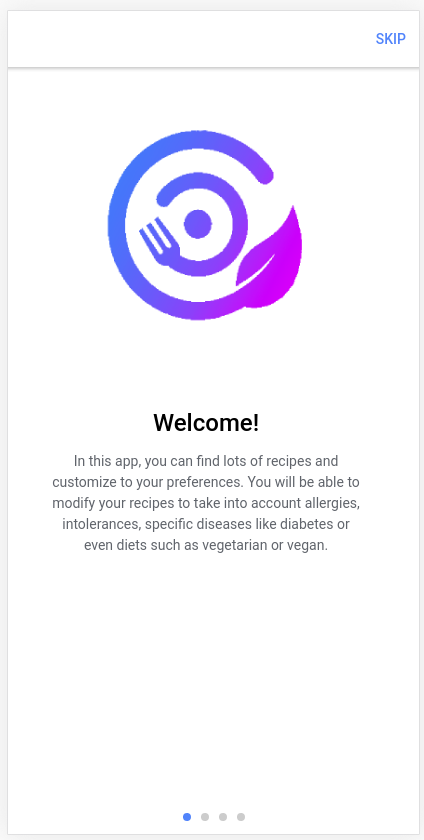
\includegraphics[width=\linewidth]{imagenes/app/pantallas/app_tutorial1.png}
        \caption{Pantalla tutorial I}
        \label{fig:app_tutorial1}
    \end{subfigure}
    \begin{subfigure}[b]{0.31
    \linewidth}
        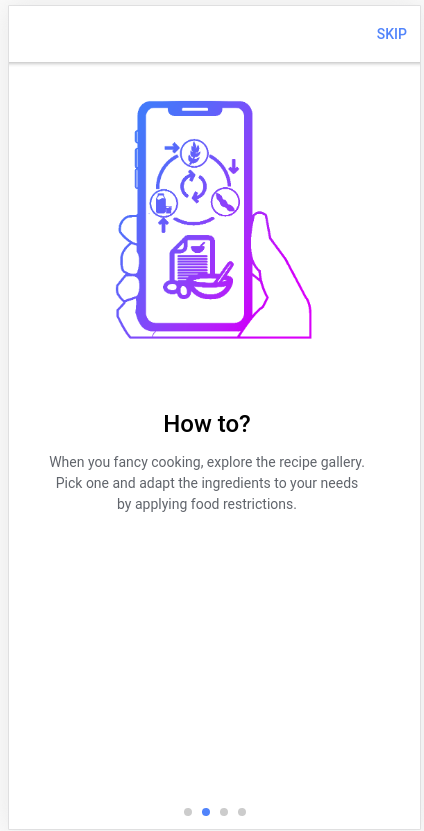
\includegraphics[width=\linewidth]{imagenes/app/pantallas/app_tutorial2.png}
        \caption{Pantalla tutorial II}
        \label{fig:app_tutorial2}
    \end{subfigure}
        \begin{subfigure}[b]{0.31
        \linewidth}
        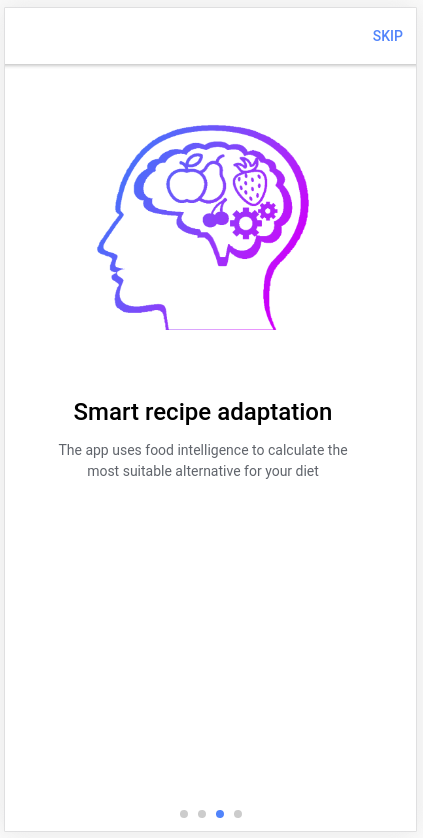
\includegraphics[width=\linewidth]{imagenes/app/pantallas/app_tutorial3.png}
        \caption{Pantalla tutorial III}
        \label{fig:app_tutorial3}
    \end{subfigure}
    \caption{Pantallas de inicio a la aplicación I}
    \label{fig:pantallas_inicio1}
\end{figure}

Una vez que se pulsa el botón \texttt{LET'S COOK} en la pantalla de bienvenida, se accede a las distintas colecciones de recetas en las que se organizan las recetas (ver Figura \ref{fig:app_coleccion}). Esta pantalla se corresponde con la pantalla de inicio de la aplicación. En dicha pantalla se muestran tres pestañas en la barra inferior: \textit{Recipes} (en la que se muestra la pantalla inicial), \textit{Search} (la cual permite realizar búsquedas sobre todas las recetas de la base de datos) y \textit{Adapted Recipes}, que contiene recetas ya adaptadas que se han querido almacenar para uso posterior.

\begin{figure}[H]
    \centering
    \begin{subfigure}[b]{0.32\linewidth}
        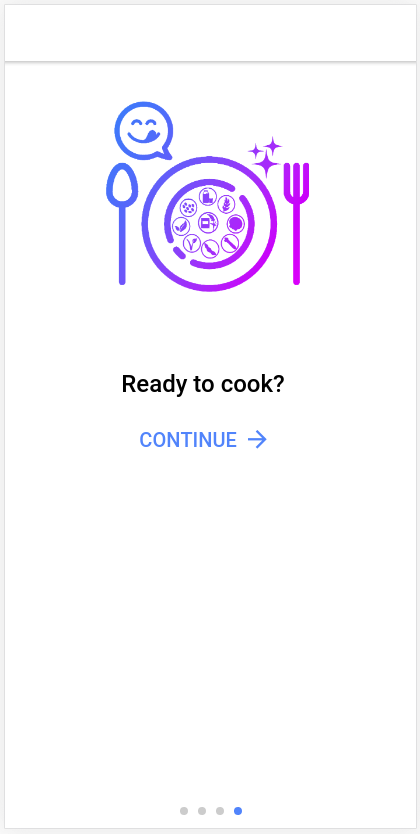
\includegraphics[width=\linewidth]{imagenes/app/pantallas/app_tutorial4.png}
        \caption{Pantalla tutorial IV}
        \label{fig:app_tutorial4}
    \end{subfigure}
    \begin{subfigure}[b]{0.32\linewidth}
        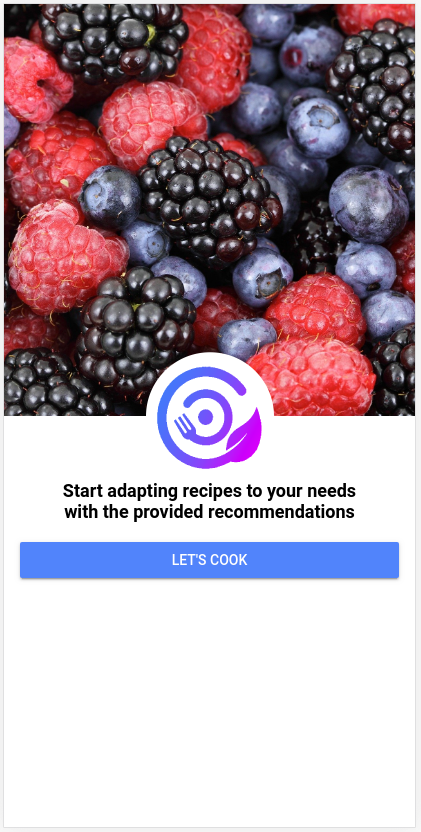
\includegraphics[width=\linewidth]{imagenes/app/pantallas/app_welcome.png}
        \caption{Pantalla bienvenida}
        \label{fig:app_welcome}
    \end{subfigure}
        \begin{subfigure}[b]{0.32\linewidth}
        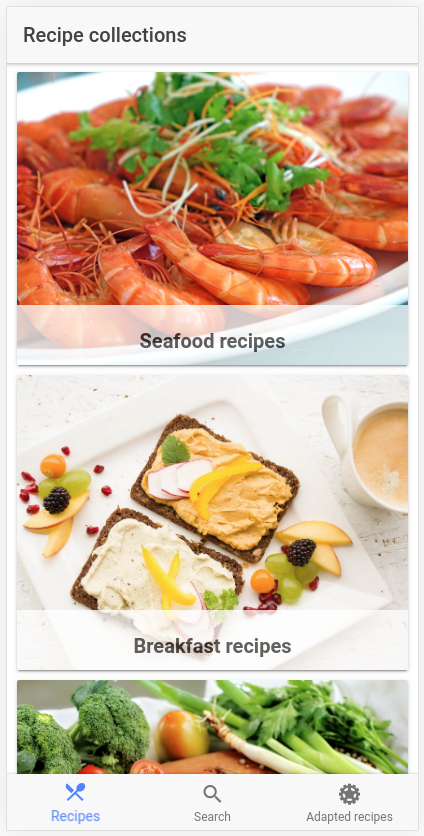
\includegraphics[width=\linewidth]{imagenes/app/pantallas/app_1.png}
        \caption{Colecciones}
        \label{fig:app_coleccion}
    \end{subfigure}
    \caption{Pantallas de inicio a la aplicación II}
    \label{fig:pantallas_inicio2}
\end{figure}

Para acceder a una receta concreta se pueden seguir dos formas: seleccionar una colección de las mostradas en la pantalla principal (ver Figura \ref{fig:app_5}) o a través de la pantalla del buscador de recetas (ver Figura \ref{fig:app_6}). Una vez que se está en la vista detallada de una receta (ver Figura \ref{fig:ejemplo1_}) ya podemos proceder a su adaptación mediante el botón azul \texttt{ADAPT}. Una vez que se indica la restricción a aplicar sobre la receta (ver Figura \ref{fig:app_7}) se facilita una pantalla intermedia que muestra la adecuación de los ingredientes a la restricción (ver Figura \ref{fig:ejemplo2_}). En esta última pantalla, se facilitan alternativas a cada ingrediente no compatible con la dieta para proceder a su modificación (ver Figura \ref{fig:ejemplo3_}). Una vez seleccionadas las alternativas a los alimentos que deben modificarse, se muestra la receta adaptada con los cambios tanto los ingredientes como los pasos de preparación que se tendrían que variar (ver Figuras \ref{fig:app_9} y \ref{fig:app_8}). 

\begin{figure}[H]
    \centering
    \begin{subfigure}[b]{0.32\linewidth}
        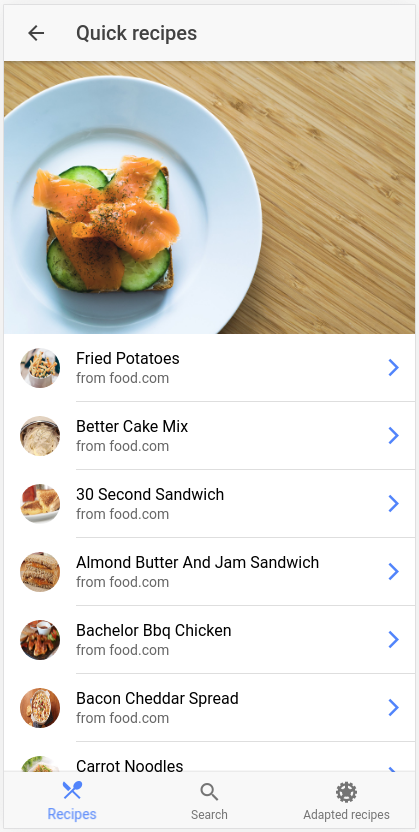
\includegraphics[width=\linewidth]{imagenes/app/pantallas/app_5.png}
        \caption{Recetas en colección}
        \label{fig:app_5}
    \end{subfigure}
    \begin{subfigure}[b]{0.319\linewidth}
        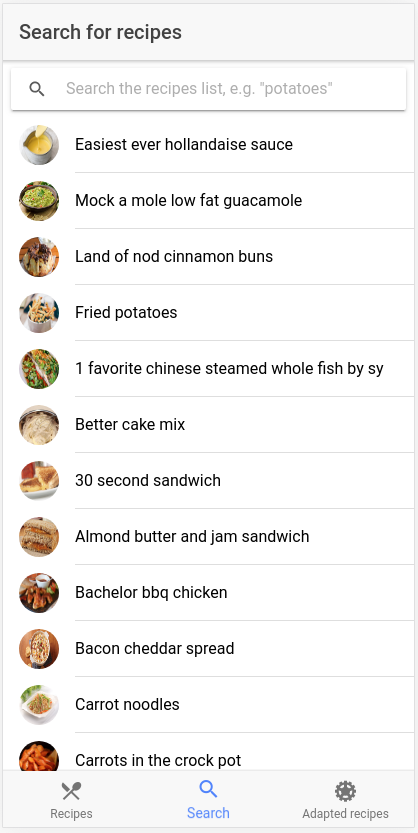
\includegraphics[width=\linewidth]{imagenes/app/pantallas/app_6.png}
        \caption{Buscador de recetas}
        \label{fig:app_6}
    \end{subfigure}
        \begin{subfigure}[b]{0.32\linewidth}
        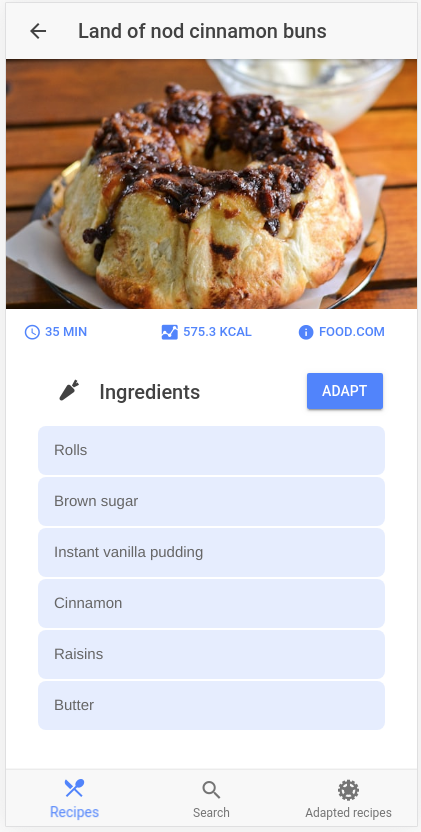
\includegraphics[width=\linewidth]{imagenes/app/pantallas/ejemplo1.png}
        \caption{Vista de receta}
        \label{fig:ejemplo1_}
    \end{subfigure}
    \caption{Pantallas para adaptar recetas}
    \label{fig:pantallas_inicio3}
\end{figure}

\begin{figure}[H]
    \centering
    \begin{subfigure}[b]{0.32\linewidth}
        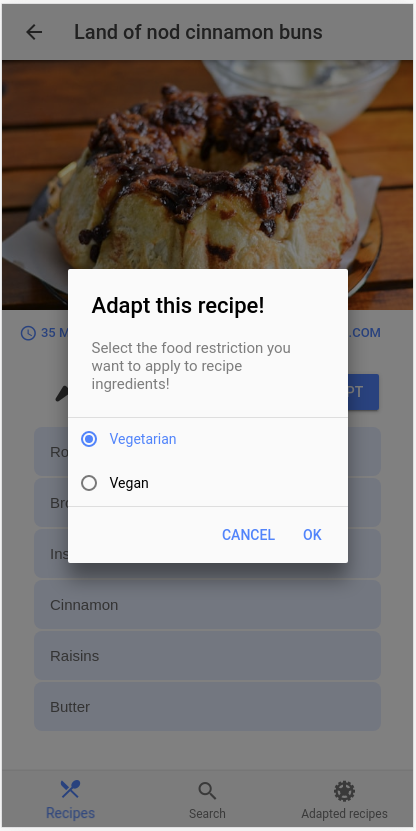
\includegraphics[width=\linewidth]{imagenes/app/pantallas/app_7.png}
        \caption{Adaptar receta I}
        \label{fig:app_7}
    \end{subfigure}
    \begin{subfigure}[b]{0.3235
    \linewidth}
        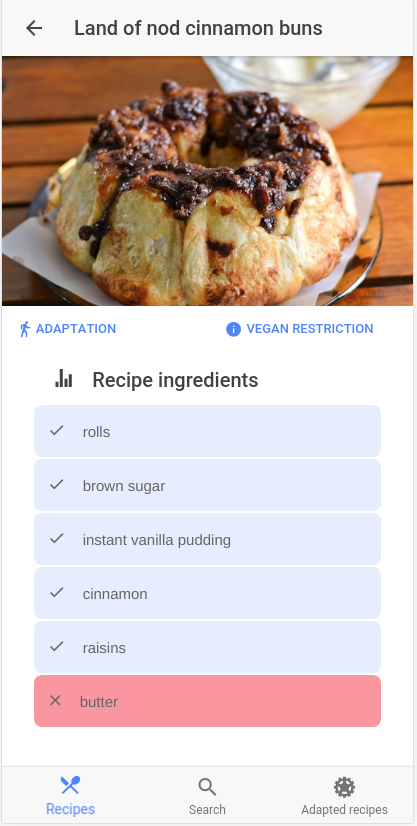
\includegraphics[width=\linewidth]{imagenes/app/pantallas/ejemplo2.png}
        \caption{Adaptar receta II}
        \label{fig:ejemplo2_}
    \end{subfigure}
        \begin{subfigure}[b]{0.32\linewidth}
        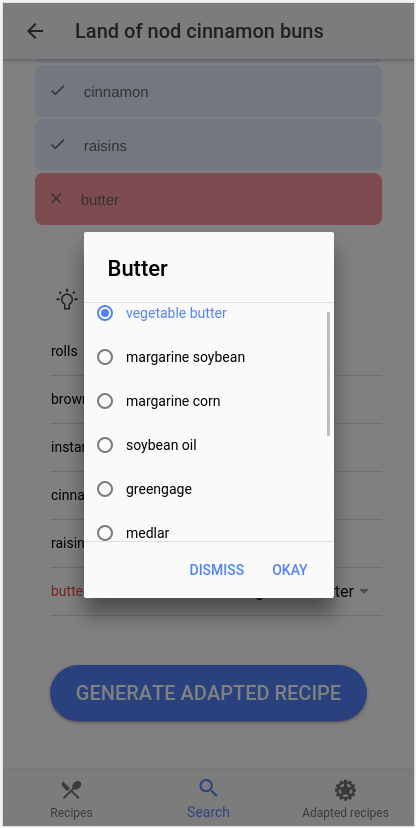
\includegraphics[width=\linewidth]{imagenes/app/pantallas/ejemplo3.png}
        \caption{Adaptar receta III}
        \label{fig:ejemplo3_}
    \end{subfigure}
    \caption{Pantallas de navegación de recetas}
    \label{fig:pantallas_inicio4}
\end{figure}

Finalmente, arriba a la derecha en la pantalla de la receta adaptada (ver Figura \ref{fig:app_8}) hay un botón que permite guardar la receta adaptada en una colección dedicada para ello (ver Figura \ref{fig:app_10}).

\begin{figure}[H]
    \centering
    \begin{subfigure}[b]{0.32\linewidth}
        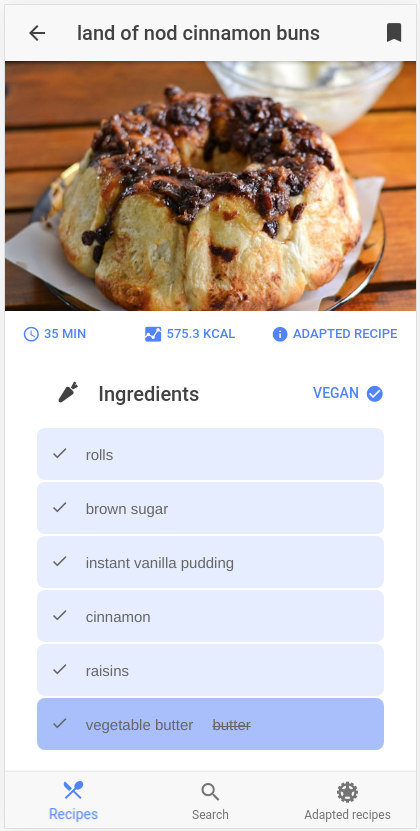
\includegraphics[width=\linewidth]{imagenes/app/pantallas/app_8.png}
        \caption{Receta adaptada I}
        \label{fig:app_8}
    \end{subfigure}
    \begin{subfigure}[b]{0.32\linewidth}
        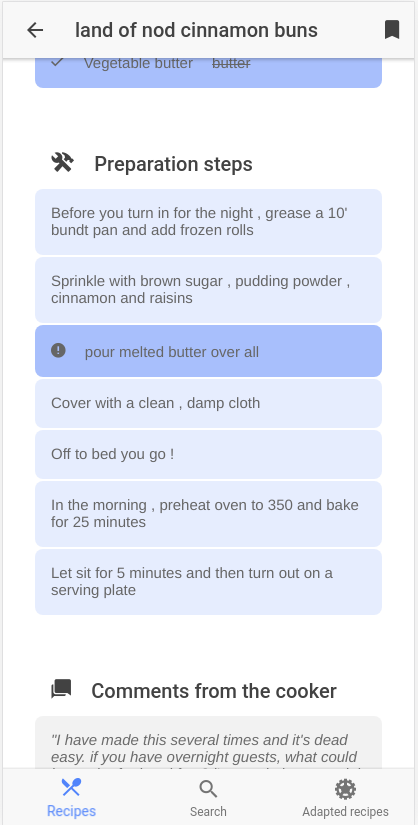
\includegraphics[width=\linewidth]{imagenes/app/pantallas/app_9.png}
        \caption{Receta adaptada II}
        \label{fig:app_9}
    \end{subfigure}
        \begin{subfigure}[b]{0.32\linewidth}
        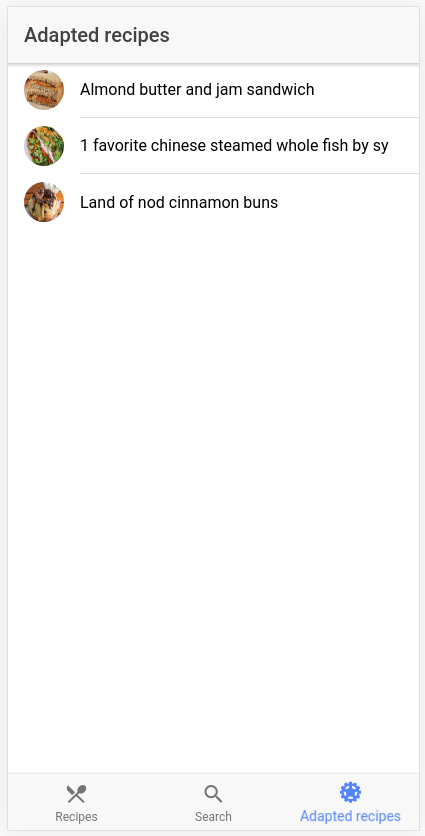
\includegraphics[width=\linewidth]{imagenes/app/pantallas/app_10.png}
        \caption{Recetas adaptadas}
        \label{fig:app_10}
    \end{subfigure}
    \caption{Pantallas de la receta adaptada}
    \label{fig:pantallas_inicio5}
\end{figure}
